\documentclass[a4paper,oneside]{scrartcl} %twocolumn,
\usepackage[utf8]{inputenc} %für MAC: applemac; für Windows: latin1 statt utf8
\usepackage[T1]{fontenc}
\usepackage[ngerman]{babel}

\usepackage{amsmath}
\usepackage{amsfonts}
\usepackage{amssymb}

\usepackage{mathptmx}
\usepackage{microtype}
\usepackage[nice]{nicefrac}

\usepackage{booktabs}
\usepackage{graphicx}
\usepackage{hyperref}
\usepackage{wrapfig}
\usepackage{float}
\usepackage{braket}

\setkomafont{captionlabel}{\upshape\bfseries}
\setkomafont{caption}{\itshape}


\title{Optisches Pumpen}
\author{Robi Pedersen \and Simon Schmeißer}
\date{Versuchsdurchführung 21.03. - 03.04.2011}

\hypersetup{
pdftitle={Optisches Pumpen},
pdfauthor={Robi Pedersen, Simon Schmeißer}}

\providecommand{\e}[1]{\ensuremath{\times 10^{#1}}}

\begin{document}
\begin{titlepage}
  \maketitle
  \vfill
  \thispagestyle{empty}
\end{titlepage}

\renewcommand*\contentsname{Table Of Contents}
\tableofcontents
\clearpage
%*****************************************************************

\section{Assignments}

\begin{itemize}
\item Acquisition of the hyperfine spectrum of the $^2S_{1/2}-^2P_{1/2}$ transition for $^{85}Rb$ and $^{87}Rb$
\item Determination of the nuclear spin of  $^{85}Rb$ and $^{87}Rb$ via double resonance
\item Determination of the earth's horizontal and vertical magnetic field via double resonance
\item Observation of the spin precession around different vertical magnetic fields
\item Determination of the relaxation time using Dehmelt's and Franzen's method
\end{itemize}
\section{Theoretische Grundlagen}


\subsection{Radioaktivität}
\subsubsection{$\alpha$-Zerfall}

Zerfällt ein sogenannter Mutterkern $_Z^AX$ in einen Tochterkern $_{Z-2}^{A-4}Y$ und ein $He^{2+}$-Ion so spricht man von $\alpha$-Zerfall. Das $He^{2+}$-Teilchen wird $\alpha$-Teilchen genannt. Die Emission von $\alpha$-Teilchen ist ein quantenmechanischer Prozess, der durch Tunneln des $\alpha$-Teilchens durch die Potentialbarriere des Coulombpotentials des Kerns ermöglicht wird. $\alpha$-Teilchen zeigen ein diskretes Spektrum. Der $\alpha$-Zerfall ist für den Versuch nicht von Relevanz.

\subsubsection{$\beta$-Zerfall}

Man unterscheidet beim $\beta$-Zerfall zwischen $\beta^+$- und $\beta^-$-Zerfall und dem Elektroneneinfang.

\begin{figure}[H]
	\begin{minipage}{0.5\textwidth}
	\centering 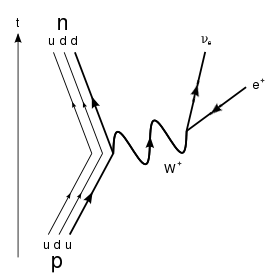
\includegraphics[width=\textwidth]{BilderTheorie/betaplus.png}
	\caption{$\beta^+$-Zerfall [en.wikipedia.org]}
	\end{minipage}
	\begin{minipage}{0.5\textwidth}
	\centering 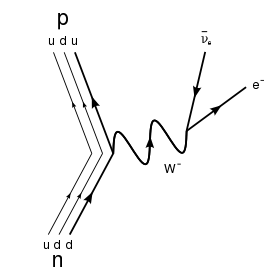
\includegraphics[width=\textwidth]{BilderTheorie/betaminus.png}
	\caption{$\beta^-$-Zerfall  [en.wikipedia.org]}	
	\end{minipage}
\end{figure}

Der $\beta^+$-Zerfall ist die Umwandlung eines Protons in ein Neutron mit Emission eines Positrons und eines Elektronenneutrinos:

$$ \beta^+: p^+ \rightarrow n^0 + e^+ + \nu_e $$

Dieser Zerfall ist wichtig für den Versuch, da auf diese Art Positronen erzeugt werden können, die mit Elektronen einen gebundenen Zustand eingehen können, nämlich das Positronium, welches in \ref{1} näher behandelt wird.
Der $\beta^-$-Zerfall ist die Umwandlung eines Neutrons in ein Proton, unter Emission eines Elektrons und eines Elektronen-Antineutrinos:

$$ \beta^-: n^0 \rightarrow p^+ + e^- + \bar \nu_e $$

Der $\beta^+$-Zerfall ist nur möglich für Protonen in einem Kern, da durch die Bindungsenergie die für den Prozess nötige Energie aufgebracht werden kann. Freie Protonen sind stabil.

Als weitere Art des $\beta$-Zerfall zählt man noch den Elektroneneinfang (EC, \emph{electron capture)}. Dieser kann stattfinden, wenn ein Elektron der untersten Schale (K-Schale), wegen dessen Aufenthaltswahrscheinlichkeit im Kern, vom Kern eingefangen wird und mit einem Proton zu einem Neutron reagiert. Dabei wird ein Elektronenneutrino emittiert:

$$ EC: p^+ + e^- \rightarrow n^0 + \nu_e $$

Der Elektroneneinfang gewinnt mit größeren Kernzahlen an Bedeutung, da dann die Aufenthaltswahrscheinlichkeit im Kern immer größer wird.

\subsubsection{$\gamma$-Zerfall}

Beim $\alpha$- und $\beta$-Zerfall gehen die Mutterkerne mit bestimmten Wahrscheinlichkeiten in verschiedene Anregungszustände der Tochterkerne über. Letztere zerfallen innerhalb einer sehr kurzen Zeit ($\sim 10^{-9}$ bis $10^{-12} s$) in den Grundzustand und emittieren dabei ein Photon mit Energien über 120 keV genannt $\gamma$-Quanten. Dieses $\gamma$-Quant wird entweder direkt vom Kern emittiert oder kann durch innere Konversion oder den Auger-Effekt seine Energie an Elektronen abgeben.

\subsection{Wechselwirkung von Photonen mit Materie \label{2}}

\subsubsection{Das Absorptionsgesetz}

Ein Photonenstrahl der einfallenden Intensität $I_0$ nimmt exponentiell mit der Dicke x einer durchquerten Materieschicht an Intensität ab. Es gilt also:

$$ I = I_0\cdot e^{-\mu x} $$

wobei $\mu$ der mediumabhängige (und photonenenergieabhängige) Absorptionkoeffizient ist. $\mu$ lässt sich als Summe der Absorptionskoeffizienten aller möglichen Wechselwirkungen von Photonen mit Materie schreiben, nämlich des Photoeffekts, des Compton-Effekts und der Paarbildung.

$$\mu = \mu_{Ph.} + \mu_{C} + \mu_{PB} $$

\subsubsection{Der Photoeffekt}

\begin{figure}[H]
	\begin{minipage}{0.59\textwidth}
	\centering 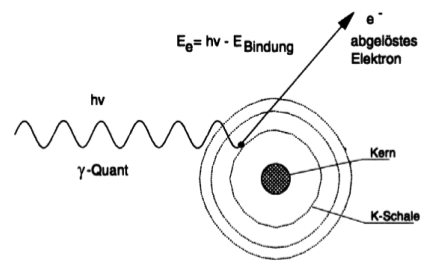
\includegraphics[width=\textwidth]{BilderTheorie/Photoeffekt.png}
	\caption{Photoeffekt}
	\end{minipage}
	\begin{minipage}{0.4\textwidth}
	Wenn ein $\gamma$-Quant ein Elektron aus der Atomhülle herausschlägt, spricht man vom Photoeffekt. Dieser Effekt tritt nur an gebundenen Elek\-tro\-nen auf. Die Energie des Photons geht zum größten Teil auf das Elektron, ein Teil wird jedoch als Rückstoßenergie vom Atom aufgenommen. Die Ab\-sorp\-tions\-wahrscheinlichkeit ist am größten in der K-Schale, also näher beim Kern. Der Photoeffekt dominiert gegenüber den anderen Effekten vor allem bei großen Atomen und Energien unter 100keV des Photons. Die entstandene Lücke wird dann durch ein weniger stark gebundenes oder freies Elektron aufgefüllt, wobei die Differenz der Bindungsenergien als Photon emittiert wird.
	\end{minipage}
\end{figure}

\subsubsection{Der Compton-Effekt}

\begin{figure}[H]
	\begin{minipage}{0.4\textwidth}
	Trifft ein Photon auf ein leicht gebundenes oder freies Elektron, so wird das Photon nicht ganz absorbiert, sondern gibt einen Teil seiner Energie an das Elektron ab und wird selbst gestreut. Durch die Streuung verliert das Photon somit an Energie, d.h. die Frequenz des gestreuten Quants ist kleiner. Der Compton-Effekt dominiert bei Energien zwischen 100 keV und einigen MeV.
	\end{minipage}
	\begin{minipage}{0.59\textwidth}
	\centering 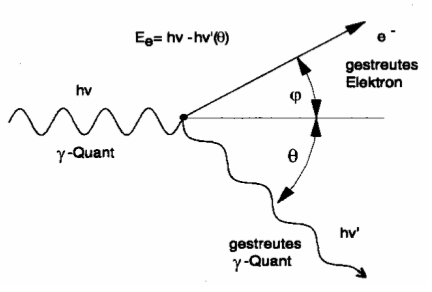
\includegraphics[width=\textwidth]{BilderTheorie/Comptoneffekt.png}
	\caption{Comptoneffekt}
	\end{minipage}

\end{figure}

\subsubsection{Die Paarbildung}

\begin{figure}[H]
	\begin{minipage}{0.5\textwidth}
	\centering 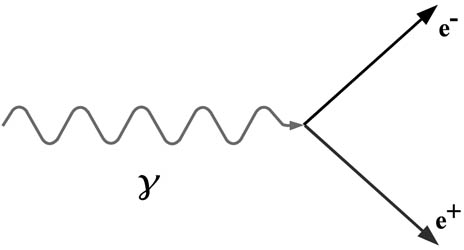
\includegraphics[width=\textwidth]{BilderTheorie/Paarbildung.jpg}
	\caption{Paarbildung}
	\end{minipage}
	\begin{minipage}{0.5\textwidth}
	Hat der $\gamma$-Quant mindestens die doppelte Ruheenergie eines Elektrons, also 1.022 MeV, so kann dieses im Feld eines Atomkerns (Stoßpartner für die Energie-Impuls-Erhaltung) ein Elektron-Positron-Paar erzeugen. 
	\end{minipage}
\end{figure}


\subsection{Szintillationszähler}

\begin{figure}[H]
	\centering 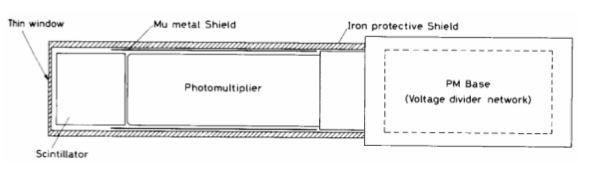
\includegraphics[width=\textwidth]{BilderTheorie/Szinti.png}
	\caption{Schema eines Szintillationszählers}
\end{figure}

Ein Szintillationszähler benutzt die in \ref{2} erklärten Ionisierungs-Phänomene um Photonen anhand geladener Strahlung nachzuweisen. Die geladene Strahlung löst Lichtblitze aus, die an einer Photokathode im Szintillator Elektronen freisetzen (Photoeffekt). Diese werden wiederum durch einen Photomultiplier verstärkt, so dass sie ein Signal mit einer messbaren Amplitude herausgeben, die der Energie des eingefallenen Quants proportional ist. Man unterscheidet zwischen organischen und anorganischen Szintillatoren. Bei dem organischen werden einzelne Moleküle angeregt, welche messbare Quanten emittieren. Beim anorganischen entstehen diese in einem Kristallgitter. Im Versuch benutzen wir anorganische NaI-Szintillationszähler.

\begin{figure}[H]
	\begin{minipage}{0.45\textwidth}
	Das Bändermodell erlaubt eine einfache Beschreibung des Verhaltens. Nämlich befinden sich bei tiefen Temperaturen alle Elektronen des Kristalls im sogenannten Valenzband. Absorbieren diese Elektronen energiereiche Strahlung, z.B. durch $\gamma$-Quanten (v.a. Photoeffekt), so werden diese angeregt und steigen auf höhere Energieniveaus. Reicht die Energie aus, so werden die Elektronen ins Leitungsband gehoben. Falls sie nicht groß genug ist um das Elektron vom Valenzband ins Leitungsband zu heben, so können sogenannte Exzitonen entstehen, lose gekoppelte Elektron-Loch-Paare (siehe Abb \ref{baendermodellszinti}). Die Exzitonen, können sich genau so wie die Leitungsband-Elektronen frei im Kristall bewegen und können unter Emission eines Photons wieder in den Grundzustand zurückkehren. 
	\end{minipage}
	\begin{minipage}{0.54\textwidth}
	\centering 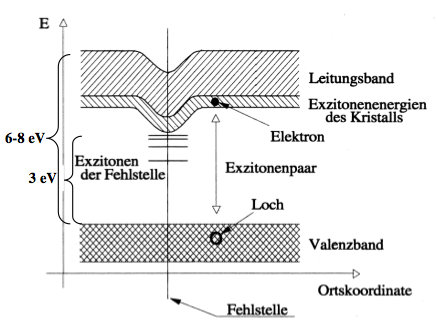
\includegraphics[width=\textwidth]{BilderTheorie/Bandmodell.png}
	\caption{Bändermodell beim NaI:Tl$^+$}
	\label{baendermodellszinti}
	\end{minipage}
\end{figure}
Eintreffende $\gamma$-Quanten haben Energien im Bereich von 0.1 bis 1 MeV, regen also mehrere hundert Elektronen gleichzeitig an. Wenn diese Elektron-Loch-Paare rekombinieren, entstehen neue Photonen, welche in den Photomultiplier geraten und dort verstärkt werden. Die Dotierung verformt lokal das Leitungsband und da diese Photonen vor allem an den Tl-Störstellen rekombinieren, reicht ihre Energie nicht aus um andere Elektronen ins Leitungsband anzuregen, somit können die Photonen nicht wieder vom Kristall absorbiert werden.


\subsection{Das Positronium \label{1}}

\begin{figure}[H]
	\begin{minipage}{0.5\textwidth}
	\centering 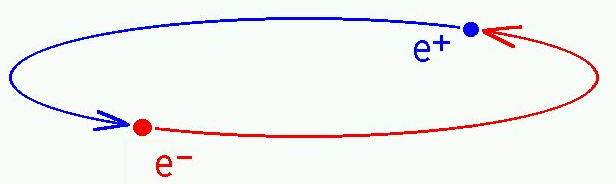
\includegraphics[width=0.9\textwidth]{BilderTheorie/Positronium.png}
	\caption{Das Positronium [cs.cdu.edu.au]}
	\end{minipage}
	\begin{minipage}{0.5\textwidth}
	Ein Positronium ist ein gebundener Zustand zwischen einem Elektron $e^-$ und dessen Antiteilchen, einem Positron $e^+$. Man kann es sich wie ein Wasserstoffatom vorstellen, bei dem das Proton durch das Positron vertauscht wurde. Der Schwerpunkt befindet sich in der Mitte der beiden Teilchen und somit ist die reduzierte Masse nur etwa halb so groß wie beim Wasserstoffatom, also genau die halbe Elektronen- bzw. Positronenmasse.
	\end{minipage}
\end{figure}
Die Energieniveaus (ohne Feinstruktur etc.) im Positronium sind also durch folgende Formel gegeben:

\begin{equation} E_n = -\frac{Ry}{2}\frac{1}{n^2} \label{3} \end{equation}

Wie man leicht nachrechnen kann, ist somit die Bindungsenergie des Grundzustands 6.8 eV, und die des 1. angeregten Zustands nur noch 1.7 eV.

\subsubsection{Erzeugung}

Ein Positron in Materie wird an den Atomen bzw. Molekülen gestreut und gibt somit einen großen Teil seiner kinetischen Energie ab. Kommt es zu einer Kollision mit einem Elektron, so annihilieren beide Teilchen. Ist die Energie des Positrons jedoch klein genug, so kann er wegen der Coulombkraft mit einem Elektron in einer äußeren Schale eines Atoms eine Bindung eingehen (Positronium), dessen Lebensdauer sich etwa im Nanosekunden-Bereich befindet und schließlich auch in einer Annihilation der beiden Teilchen endet. Mithilfe der Formel (\ref{3}), kann man erkennen, dass die Energie der Positronen über $V_i - 6.8$ eV sein muss, damit ein Positronium im Grundzustand erzeugt werden kann ($V_i$ ist die Ionisationsenergie der Atome oder Moleküle des Mediums). Die Erzeugung des 1. angeregten Zustands ist sehr unwahrscheinlich, da bei den betroffenen Energien die inelastische Streuung stark überwiegt. 

Die Annihilation unterscheidet sich je nach Spinstellung der beiden Teilchen, nämlich zerfallen sie entweder in 2 oder 3 Photonen.
Der Wirkungsquerschnitt für den 2$\gamma$-Zerfall ist gegeben durch

\begin{equation} \sigma_{2\gamma}=\frac{\pi\cdot r_0^2\cdot c}{v} \end{equation}

wobei $r_0=e^2/mc^2=2.8 fm$ der Thomson-Radius (klassischer Elektronenradius) ist und $v$ die Relativgeschwindigkeit zwischen dem Elektron und dem Positron. Der Wirkungsquerschnitt für den 3$\gamma$-Zerfall ist um $\alpha=1/137$ (Feinstrukturkonstante) kleiner. Auf die Spinstellungen und deren Unterschiede wird im nächsten Punkt näher eingegangen.

\subsubsection{Para- und Orthopositronium}

Da das Elektron und das Positron beide einen Spin von $j=1/2$ haben, können sie im gebundenen Zustand entweder zu einem Singulett oder zu einem Triplett koppeln.\\

\begin{tabular}[H]{p{4cm} p{4cm} p{4cm}}
 & Para-Positronium & Ortho-Positronium\\
 & &\\
Zustand & Singulett $^1S_0$ & Triplett $^3S_1$\\
Spineinstellung & Antiparallel, $J=0$ & Parallel, $J=1$\\
 & $m_J = 0$ & $m_J = -1,\ 0,\ 1$\\
Hauptzerfall & 2$\gamma$ & 3$\gamma$\\
Lebensdauer & $1.25\cdot 10^{-10} s$ & $1.39\cdot 10^{-7} s$\\
\end{tabular}\\

Der 1$\gamma$-Zerfall ist wegen der Impulserhaltung nicht möglich. Zerfälle in mehr als 3 Photonen sind durchaus möglich, wobei das Para-Positronium nur in eine gerade Zahl Photonen zerfallen kann und das Ortho-Positronium nur in ungerade Zahlen (siehe hierzu Kap. \ref{4}). Höhere Zerfälle sind jedoch relativ unwahrscheinlich und irrelevant für die Messung.
Der Unterschied in der Lebensdauer beträgt den Faktor:

\begin{equation} \frac{\tau_{2\gamma}}{\tau_{3\gamma}} = 1115 \end{equation}

\subsubsection{Auswahlregeln der Zerfälle \label{4}}

Um die Symmetrieauswahlregeln der Zerfälle der beiden Positronium-Zustände zu bestimmen, benutzen wir die C-Parität. Wir beweisen zuerst kurz, dass die Ladungskonjugation $\hat C$ auf ein Positronium angewandt genau die gleiche Operation macht, als würde man zuerst den Paritäts-Operator $\hat P$ und dann den Spinaustausch-Operator $\hat S$ auf das Positronium anwenden.

Man habe zum Beispiel ein Elektron am Ort $\vec r$ mit Spin $\alpha$ und ein Positron mit Ort $-\vec r$ und dem Spin $\beta$:
$$\hat S\cdot\hat P\mid e^-,\ \vec r,\ \alpha \rangle \otimes \mid e^+,\ -\vec r,\ \beta \rangle
 = p\hat S\mid e^-,\ -\vec r,\ \alpha \rangle \otimes \mid e^+,\ \vec r,\ \beta \rangle 
 = sp\mid e^-,\ -\vec r,\ \beta \rangle \otimes \mid e^+,\ \vec r,\ \alpha \rangle $$
Wie man sieht entspricht der Endzustand genau der Ladungskonjugation der beiden Teilchen, also direkt der Ersetzung der beiden Teilchen durch ihr Antiteilchen. Der Eigenwert sp entspricht somit dem Eigenwert c. Diese Ersetzung macht man, um die Eigenwerte der Ladungskonjugation zu bestimmen.

Da die Parität des Elektrons genau der Parität des Positrons entgegengesetzt ist, folgt für den Eigenwert
$$p = -(-1)^l = -1 \text{\ \ im Grundzustand (l=0)}$$
Der Eigenwert des Spinaustauschoperators ist gegeben durch $$s=(-1)^{J+1}$$
Somit ist $s=-1$ für den Singulett-Zustand und $s=1$ für den Triplett-Zustand.
Schlussendlich gilt also:

\begin{equation} \hat C \mid ^1S_0 \rangle = 1 \mid ^1S_0 \rangle \end{equation}
\begin{equation} \hat C \mid ^3S_1 \rangle = -1 \mid ^1S_0 \rangle \end{equation}

Die Photonen, die beim Zerfall ausgestrahlt werden, besitzen die C-Parität -1. Somit hat ein n-Photonen-Zerfall die Parität $(-1)^n$, was erklärt, warum der Singulett-Zustand nur in 2n Photonen und der Triplett-Zustand nur in 2n+1 Photonen zerfallen kann.

\subsubsection{Hyperfeinstruktur und Annihilationskraft}

Der Hamiltonian der ''Grobstruktur'' lautet $$H = \frac{p_{e^-}^2}{2m_e}+\frac{p_{e^+}^2}{2m_e}-\frac{e}{r^2}$$ woraus die Energiezustände in Gl. (\ref{4}) folgen. Wenn man neben der Feinstruktur auch noch die Wechselwirkungen der magnetischen Spinmomente betrachtet, die sogenannte Hyperfeinstruktur, stößt man auf eine Energieaufspaltung der Triplett und Singulettzustände im Grundzustand. Neben der Hyperfeinstruktur spielt auch noch die Annihilationskraft eine genau so große Rolle in der Aufspaltung dieser Niveaus.

\begin{itemize}

\item Hyperfeinstruktur:\\
Die Wechselwirkungsenergie der magnetischen Momente entspricht in erster Näherung
\begin{equation} W = \frac{8\pi}{3}\mu^2\sigma^-\sigma^+|\Psi(0)|^2 \end{equation}
wobei $\sigma^\pm$ die Spinzustände des Positrons/Elektrons sind und $\mu = \frac{e\hbar}{2mc}$ das Bohrsche Magneton. $\Psi(0)$ ist die Wellenfunktion am Ort des Positron und ihr Betragsquadrat ist
$$|\Psi(0)|^2 = \frac{1}{\pi}\left(\frac{-1}{2a_0}\right)^3$$
$a_0 = 0.53 \mathring A$ ist der Bohrsche Atomradius. Der Eigenwert des Spinoperators $\sigma^-\sigma^+$ beträgt für den Singulett-Zustand -3 und für den Triplett-Zustand +1. Man erhält somit die Energiebeiträge
$$W(^1S_0) = -\frac{1}{4}\alpha^4mc^2 \text{\ \ \ \ und \ \ \ \ } W(^3S_1) = \frac{1}{12}\alpha^4mc^2$$
und kann ausrechnen dass die Aufspaltung
\begin{equation} \Delta W = 4.83 \cdot 10^{-4}\ eV \end{equation} beträgt, und der Triplett-Zuständ oberhalb des Singulett-Zustands liegt.

\item Annihilationskraft:\\
\begin{figure}[H]
	\begin{minipage}{0.5\textwidth}
	Die sogenannte Annihilationskraft berücksichtigt den Fall, dass ein Elektron und ein Positron kurzzeitig in ein virtuelles Photon annihilieren können und dann wieder ein Positronium bilden können. Diese Tatsache liefert einen Energieterm für alle Zustände mit ungerader C-Parität, da nur diese in eine ungerade Zahl Photonen zerfallen können (siehe vorigen Abschnitt). Der Triplettzustand erhält hierdurch den Energiebeitrag:

\begin{equation} W_A(^3S_1)=8\pi\mu^2|\Psi(0)|^2 = \frac{1}{4}\alpha^2mc^2 \end{equation}

Der numerische Wert hierfür ist $W_A = 3.62\cdot10^{-4}$ eV und ist somit fast genau so groß wie der Term der Hyperfeinstruktur.
	\end{minipage}
	\begin{minipage}{0.5\textwidth}
	\centering 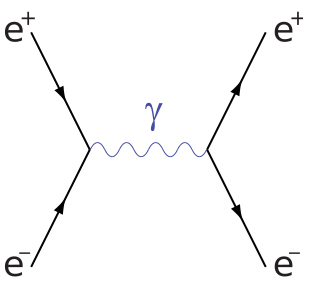
\includegraphics[width=0.8\textwidth]{BilderTheorie/epep.png}
	\caption{Feynman-Graph der Annihila\-tionskraft [howgravityworks.org]}
	\end{minipage}
\end{figure}

\item Die gesamte Aufspaltung beträgt somit 
\begin{equation} \boxed{\Delta W = \frac{7}{12}\alpha^4mc^2 = 8.45\cdot10^{-4} eV} \end{equation}
\end{itemize}

\subsection{Der Zeeman-Effekt}

Der Zeeman-Effekt beschreibt die Aufspaltung der Energiezustände eines gebundenen Zustands in einem Magnetfeld B. Man unterscheided zwischen dem normalen und dem anomalen Zeeman-Effekt. 
Der normale Zeeman-Effekt spaltet die Energieniveaus eines bestimmten Bahndrehimpulses $l$ in $2l+1$ Terme, deren Energieaufspaltung abhängig von der z-Komponente $m_l$ des Bahdrehimpulses ist:
$$\Delta E = \mu_B\cdot m_l \cdot B$$
$\mu_B$ ist hier das Bohrsche Magneton. Der normale Zeeman-Effekt ist also die Aufspaltung aufgrund des mit dem Bahndrehimpulses verknüpften magnetischen Moment in einem externen Magnetfeld.
Der anomale Zeeman-Effekt ist die zusätzliche Berücksichtigung des magnetischen Moments, das durch den Spin hervorgerufen wird. Hier muss also die $l-s$-Kopplung ($\vec J = \vec L + \vec S$) berücksichtigt werden, so dass die Aufspaltung
$$\Delta E = g_J\cdot\mu_B\cdot m_J\cdot B$$
beträgt, wobei $g_J$ der Landé-Faktor des Gesamtdrehimpulses ist.\\

Das Positronium selber hat kein magnetisches Moment, da sich das vom Elektron mit dem vom Positron genau aufhebt. Da jedoch das externe Magnetfeld im Positronium ein magnetisches Moment erzeugt, kann dieses wiederum vom Magnetfeld aufgespalten werden, so dass man einen Zeeman-Effekt 2. Ordnung erhält. Dieser ist im Allgemeinen wesentlich schwächer als der Zeeman-Effekt 1. Ordnung, ist aber beim Positronium der einzige der beiträgt. Die Wirkung des Effekts lässt sich mittels quantenmechanischer Störungstheorie berechnen. Der Störungsoperator hat die Form:

\begin{equation} V=\frac{eB}{mc}(S^- - S^+) \end{equation} 



\subsection{Das Quenching}
\subsubsection{Quantenmechanische Störungstheorie}
\subsubsection{Quenching beim Positronium}

\subsection{Signalverarbeitung}
























\section{Versuchsbeschreibung}
In diesem Versuch wird der Zerfall von Positronium untersucht. Als Quelle für die Positronen dient eine dünne Mylarfolie mit ${}^{22}Na$, welche sich in einer Gaskammer befindet. Der Stickstoff in der Kammer dient einerseits zur Thermalisierung der Positronen, bietet andererseits aber auch Elektronen für die Paarbildung. Im ersten Versuchsteil untersuchen wir den Zwei- und Drei-Photonen-Zerfall, im zweiten Versuchsteil ermitteln wir aus dem Quenching des Triplettzustandes die Aufspaltung durch Zeeman- und Annihilationskraft.

\subsection{Zerfallscharakteristik}

\begin{figure}
 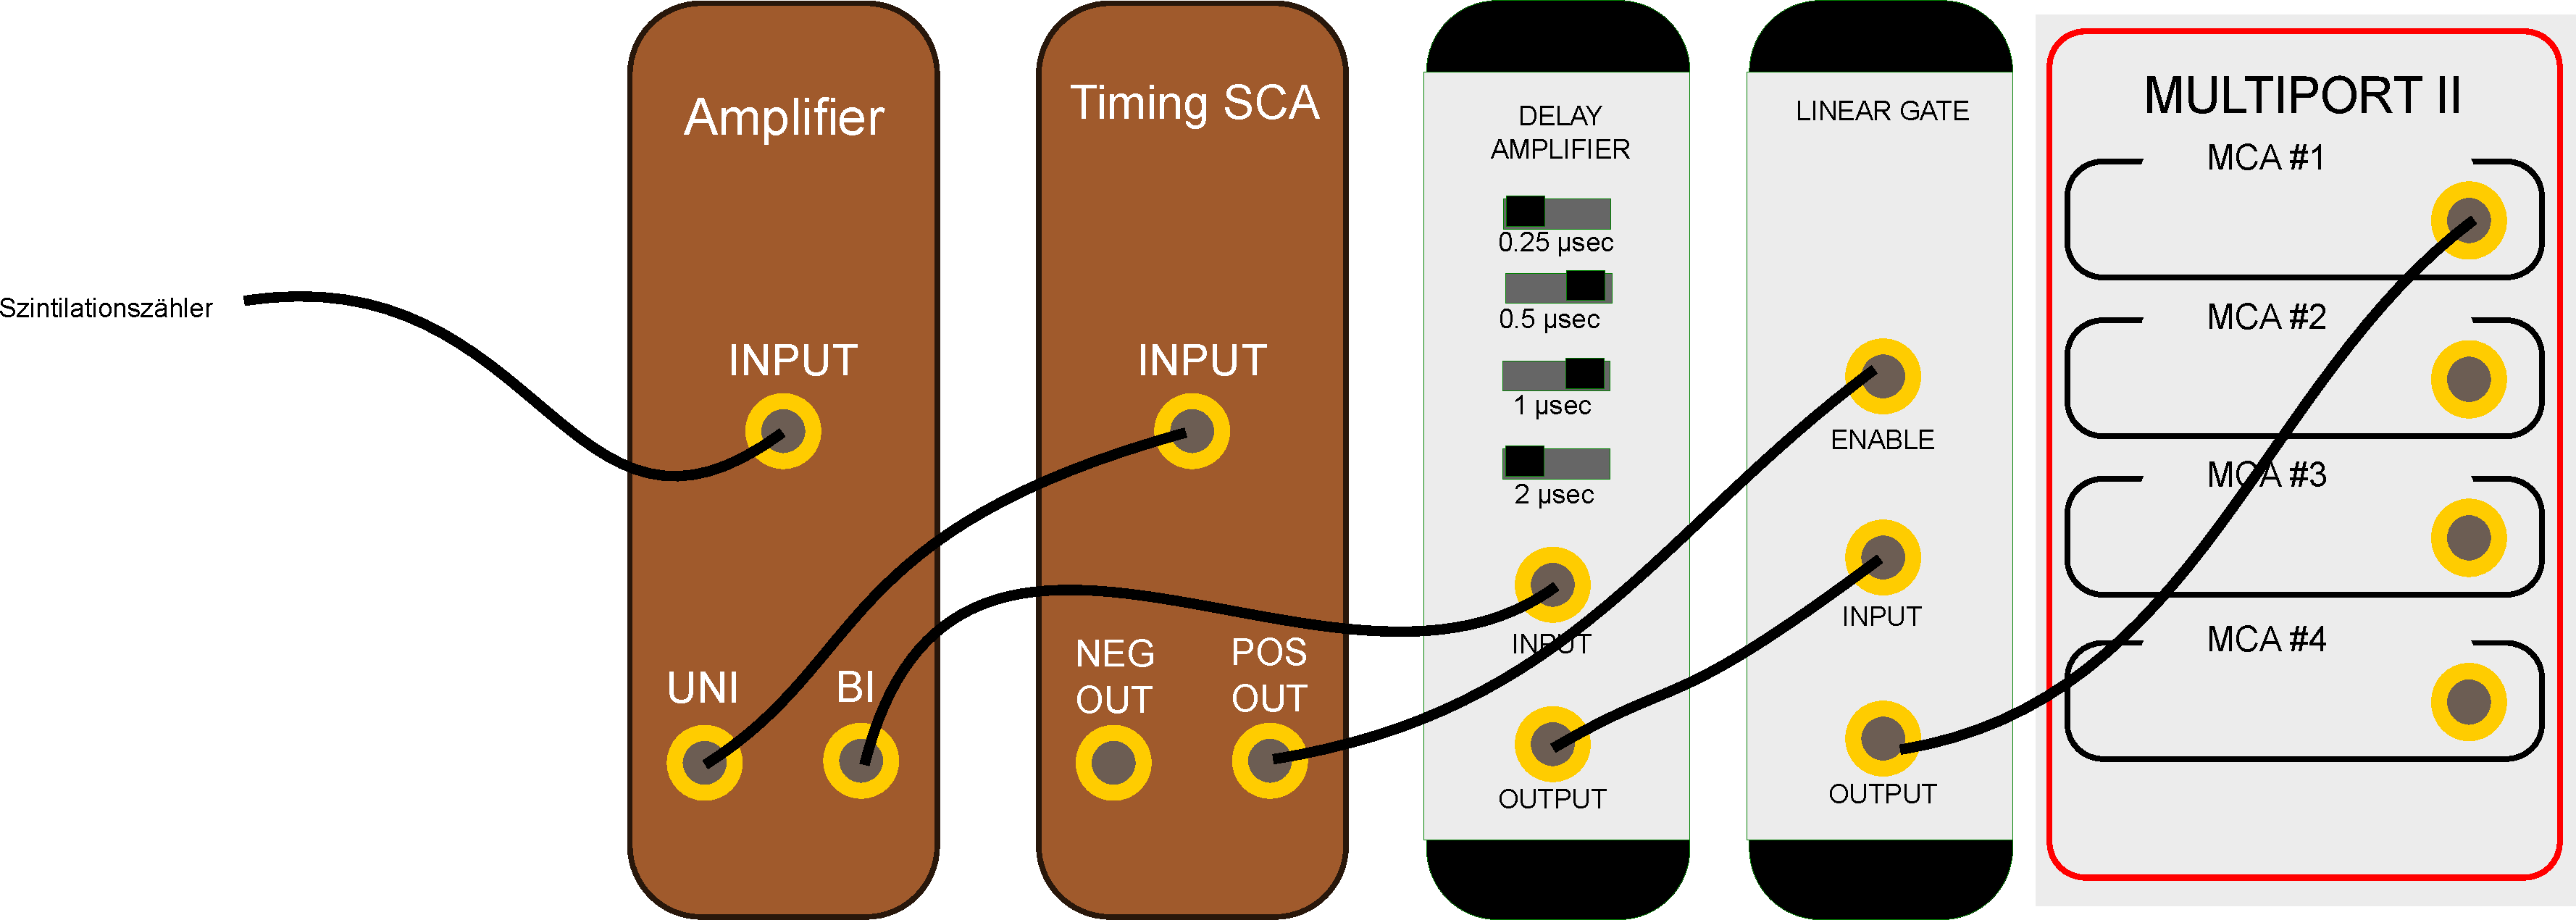
\includegraphics[width=\textwidth]{BilderAufbau/spektrum.pdf}
 \caption{Versuchsaufbau für die Messung des Spektrums und das Einstellen der Fenster}
 \label{schaltplan_sca_lin_mca}
\end{figure}

Das Zerfallsspektrum des Positroniums wird von Szintillatoren gemessen. Zur Energiekalibration wird das komplette Spektrum mit einem Multi Channel Analysator (MCA) aufgenommen. Über den 1270keV Peak des ${}^{22}Na$-Zerfalls und den 511keV Peak des Zwei-Photonen-Zerfalls kann dann eine Energieeichung des MCA ermittelt werden. Da sich die Szintillatoren verschiedene Charakteristiken zeigen, wird diese für alle durchgeführt.

\begin{figure}
 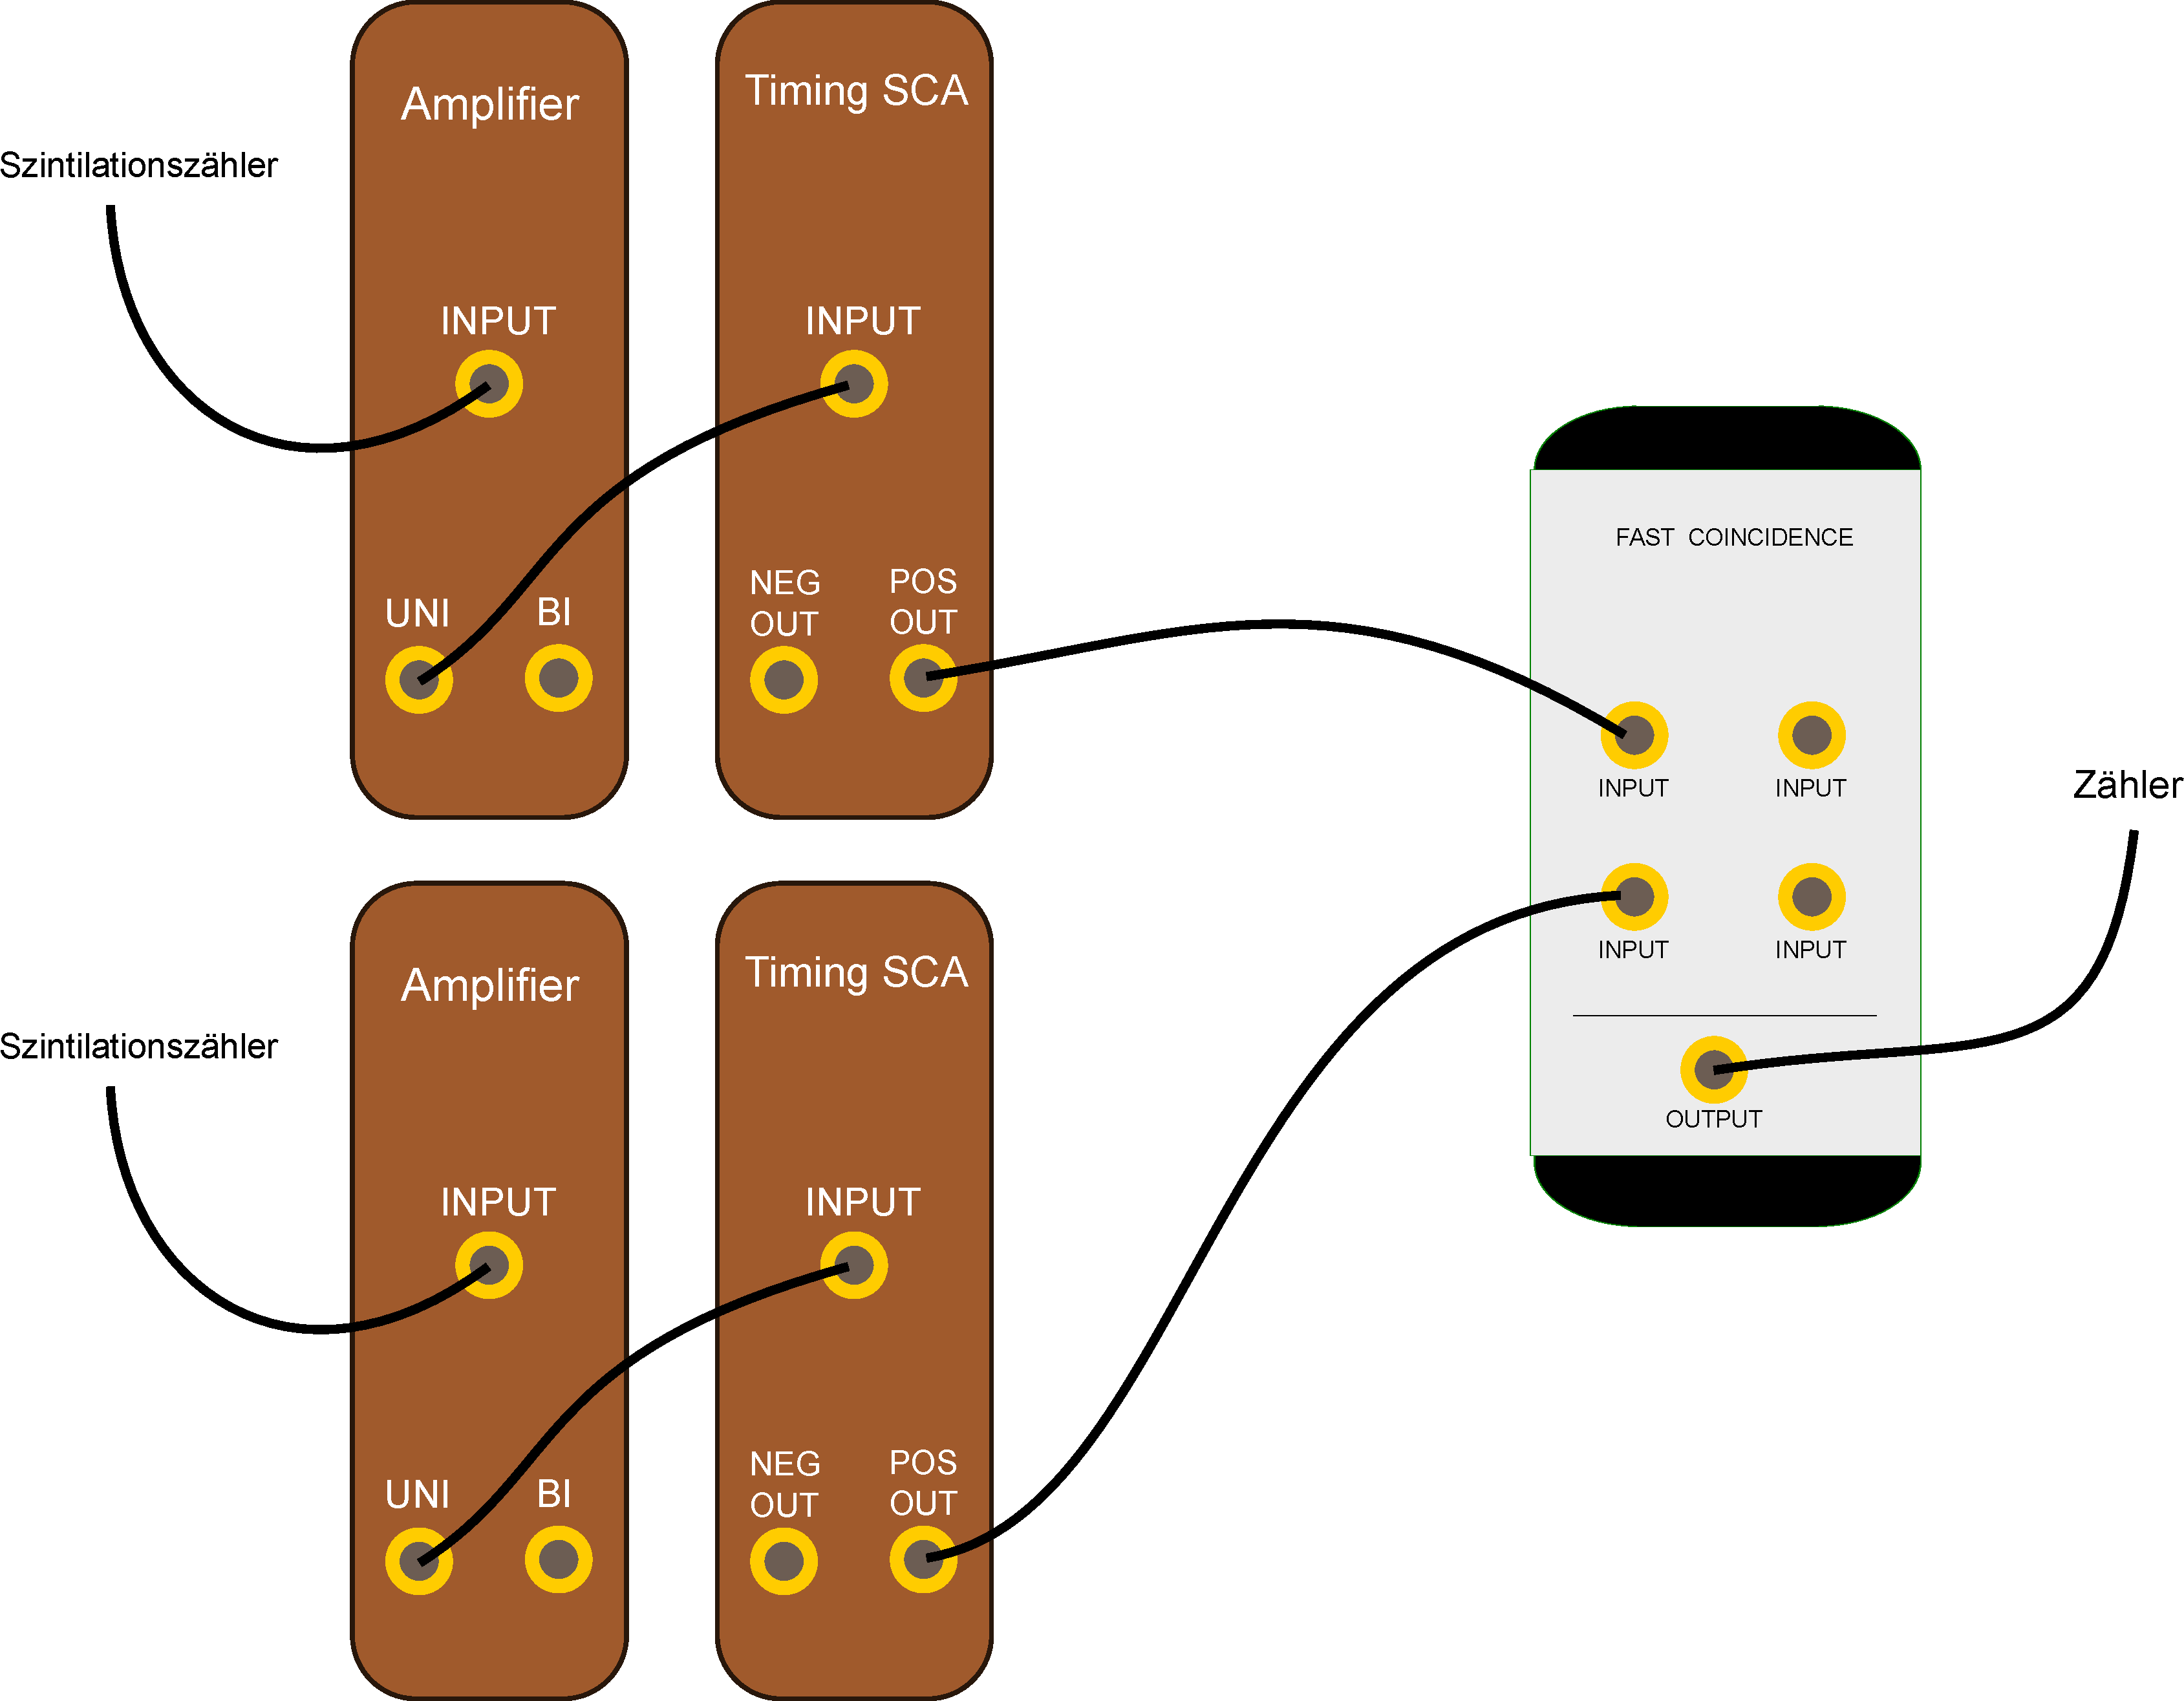
\includegraphics[width=\textwidth]{BilderAufbau/2er-koinzidenz.pdf}
 \caption{Versuchsaufbau für die Koinzidenzmessung des 2-Photonen-Zerfalls}
 \label{schaltplan_2_sca_coin_zaehler}
\end{figure}

Für die Untersuchung des Zerfalls des Singulett-Zustandes wird die Messung auf den 511keV-Peak begrenzt. Zwei der Szintillatoren werden nun in einer Ebene gegeneinader verdreht, um so die Winkelkorrelation zu untersuchen. Dabei werden die Signale zuerst mit Single Channel Analysatoren (SCA) auf den 511keV Bereich begrenzt. Mit einer Fast Coincidenze wird dann überprüft, ob beide Pulse vom selben Zerfall stammen. Die Anzahl solcher Ereignisse innerhalb eines Messintervalls wird gezählt. 


\begin{figure}
 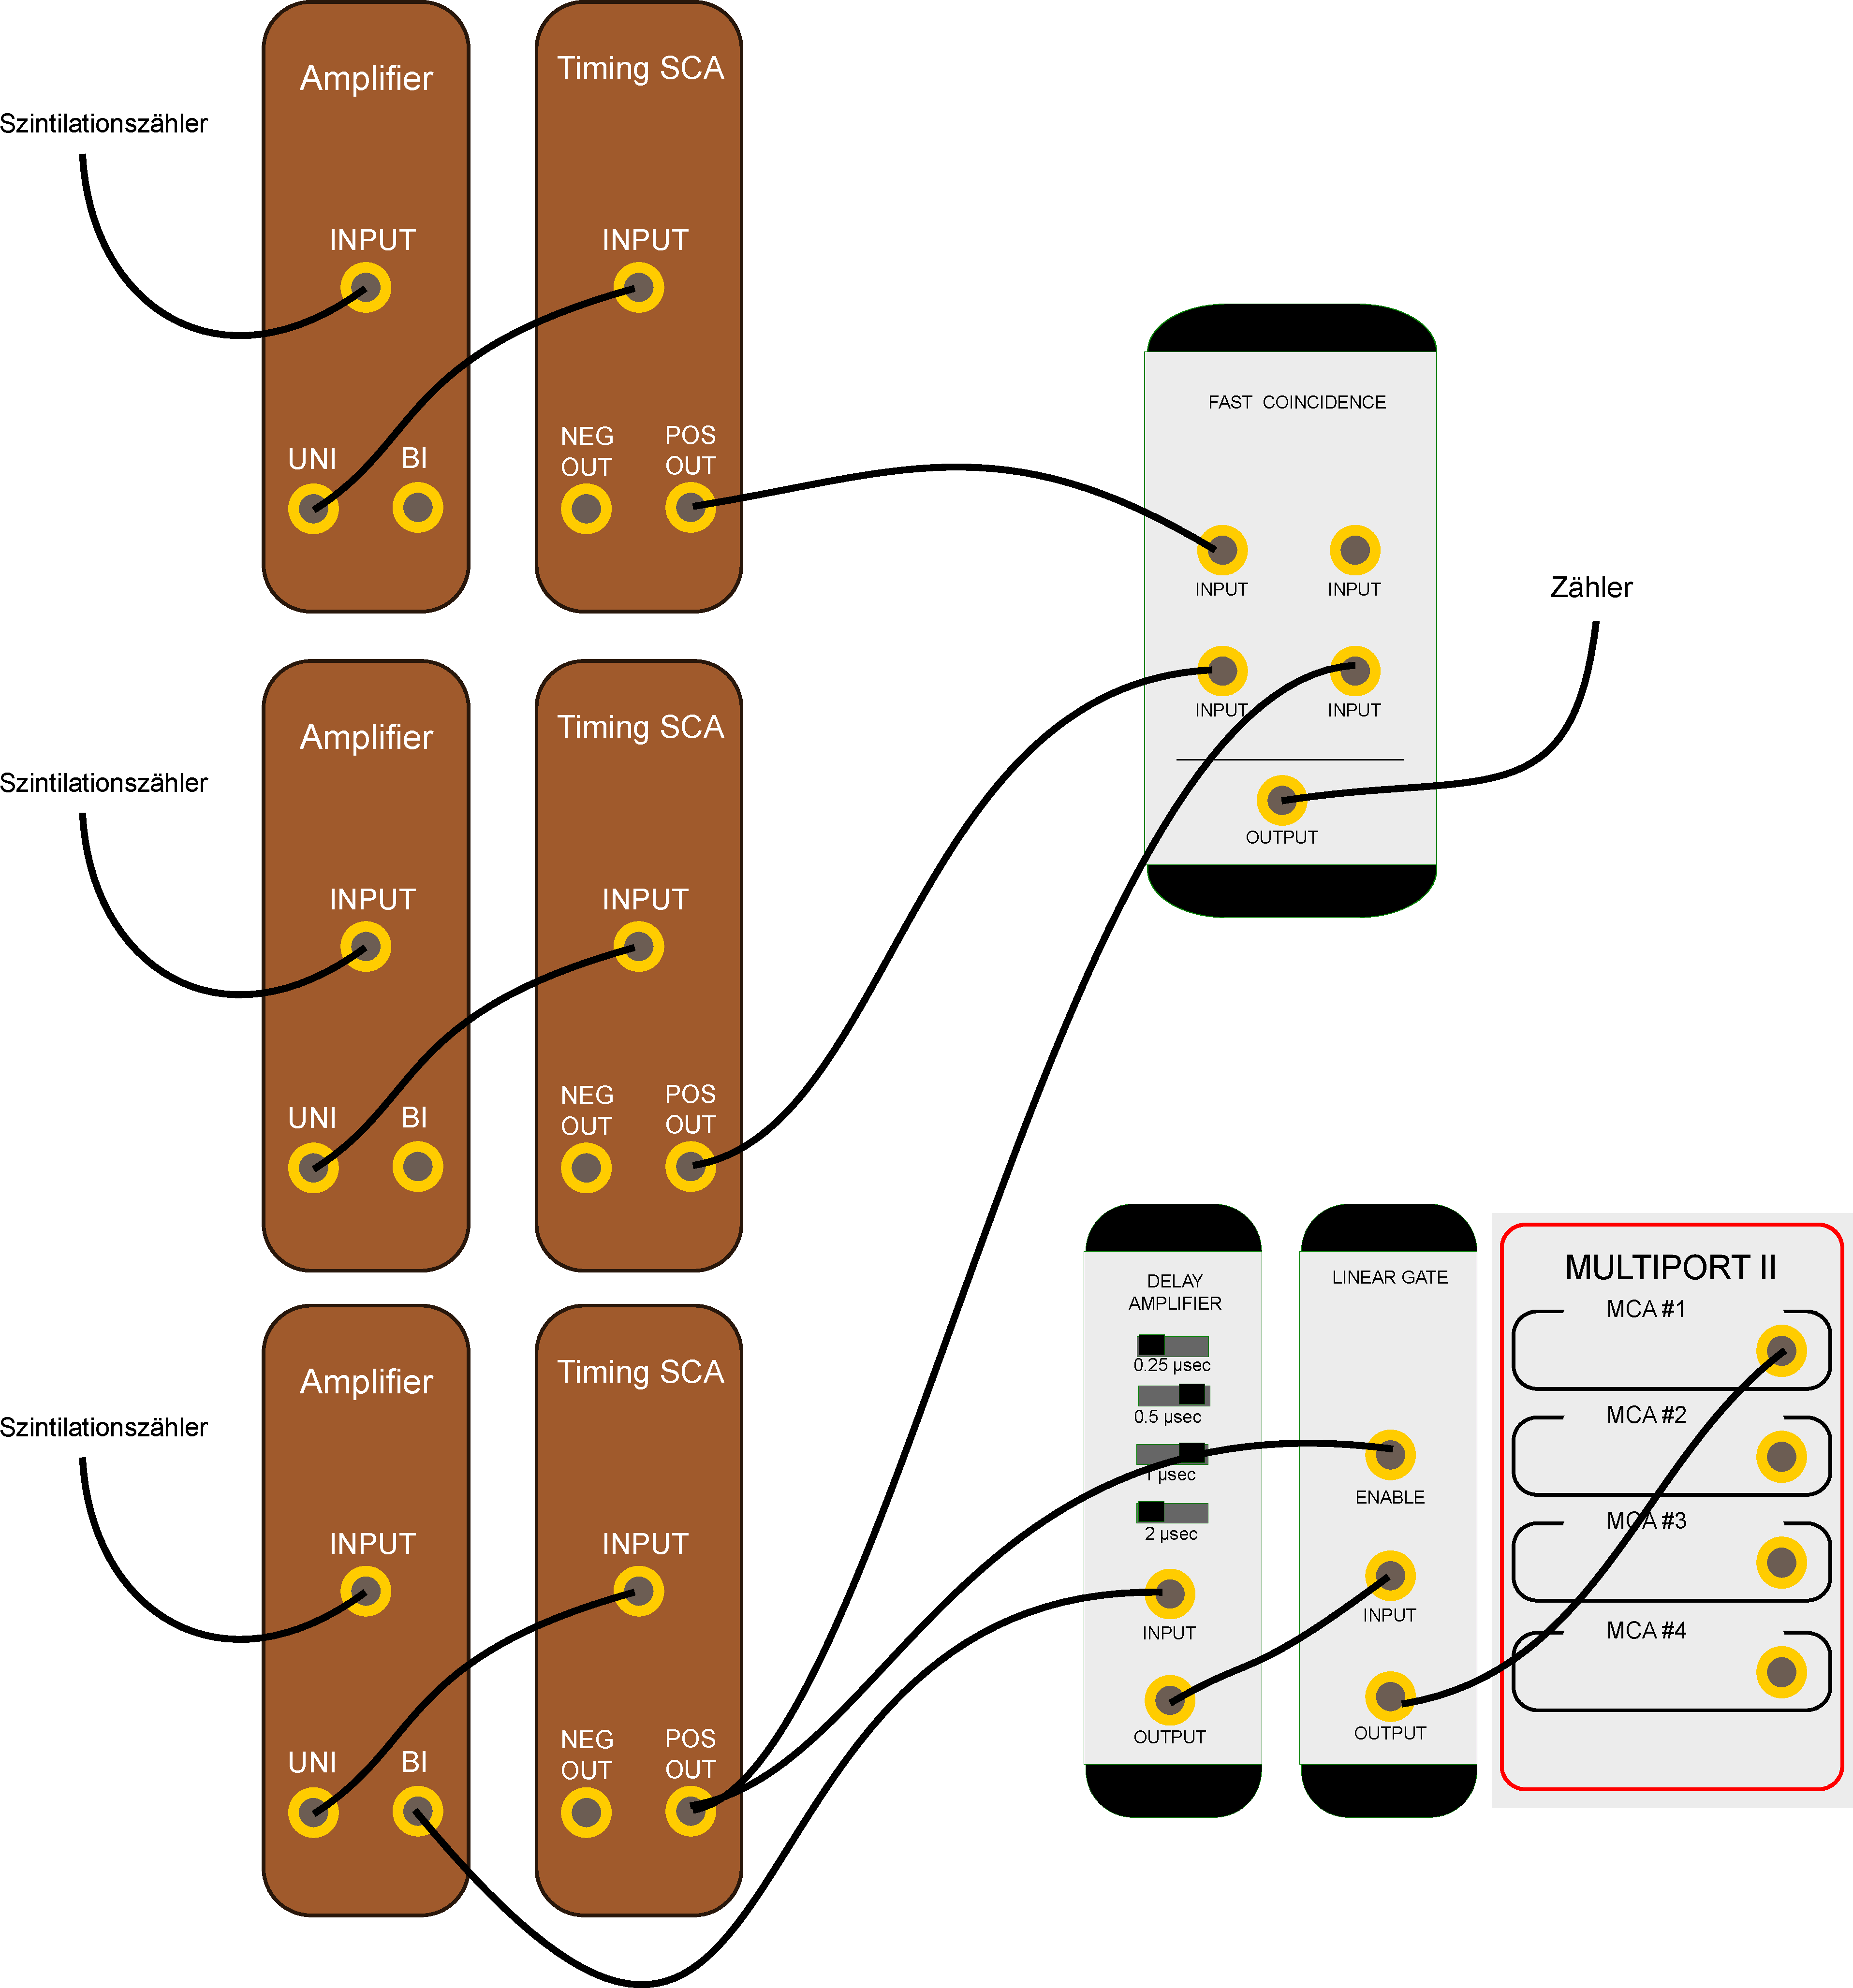
\includegraphics[width=\textwidth]{BilderAufbau/3er-koinzidenz.pdf}
 \caption{Versuchsaufbau für die Koinzidenzmessung des 3-Photonen-Zerfalls}
 \label{schaltplan_3_sca_coin_mca_zaehler}
\end{figure}

Für die Untersuchung des Drei-Photonen-Zerfalls werden drei Szintillatoren in eine $120^\circ$ Konfiguration gebracht. Bei Zweien wird mit SCAs eine Energieobergrenze unterhalb der 511keV des Singulett-Zerfalls gesetzt. Die Energie des dritten Szintillators wird nicht eingeschränkt. Mit der Fast Coinzidence wird überprüft, ob die Photonen vom selben Ereignis stammen. Das Spektrum des dritten SZ wird mit dem MCA aufgenommen. 

\subsection{Quenching}

Im zweiten Versuchsteil geht es darum die Unterdrückung des ${}^3S_0$-Zustandes durch ein Magnetfeld, genannt Quenching, zu untersuchen. Dazu wird jetzt auch beim dritten SCA ein Energiefenster von ca. $\frac{2}{3} m_0$ eingestellt. Mit einem Helmholzspulenpaar wird in der Gaskammer ein konstantes Magnetfeld erzeugt. Dieses wird über die Messreihen variiert und die Abnahme der 3er-Zerfälle registriert.
\section{Versuchsdurchführung und Auswertung}

\subsection{Verbleibende Aktivität}

Die \Na-Probe wurde laut Beschriftung am Versuchsaufbau am 29.09.1993 eingesetzt. Sie hatte damals eine Aktivität von $A_{93} = 3,7\e{6} Bq$ und die Halbwertszeit wird mit $t_{1/2} = 2,6 a$ angegeben. Somit ergibt sich für die Restaktivität:
\begin{eqnarray*}
 A(t) = & A_{93} \cdot e^{-\frac{\ln 2}{t_{\nicefrac{1}{2}}} t} \\
      \approx & 3,61\e{4} Bq
\end{eqnarray*}
\label{verbleibende_aktivitaet}
Die Messungen in der Staatsexamensarbeit wurden bei $A_{St} = 0,15\, mCurie = 5,55\e{6} Bq$ durchgeführt. Wir erwarten also dass die Rate der Ereignisse im Experiment bei uns in etwa zwei Größenordnungen kleiner sein wird. Für die statistische Genauigkeit der Messungen ist dies nicht von Vorteil.

\subsection{Szintillatorspektren}
Wir haben das Spektrum des \Na  mit jedem der drei Szintillatoren aufgenommen (siehe Abb. \ref{22na-schrottspektrum}). Dazu haben wir je einen direkt an den Multi Channel Analysator (MCA) angeschlossen und 20 min gemessen.

\begin{figure}[ht]
 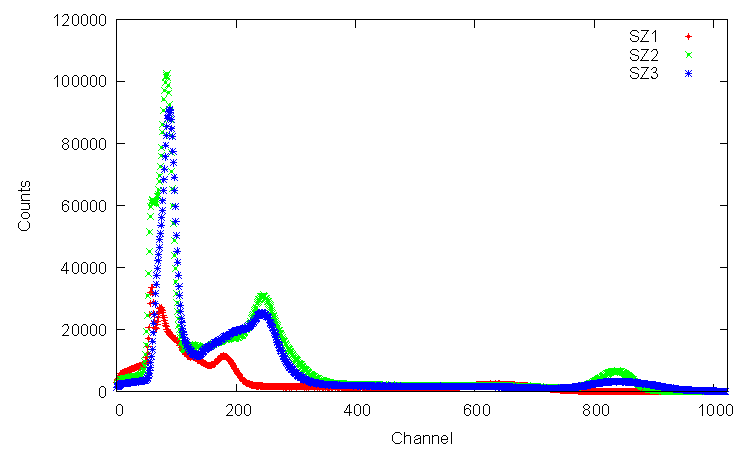
\includegraphics[width=\textwidth]{Graphen/Na-Spektren/na-spektren-1.pdf}
 \caption{Spektrum des \Na-Zerfalls, aufgenommen mit drei ungefilterten Szintilatoren}
 \label{22na-schrottspektrum}
\end{figure}

Dabei haben wir folgende Verstärkungen eingestellt:

\begin{tabular}{lr}
SZ1:& 8,13\\
SZ2:& 5,00\\
SZ3:& 10,00
\end{tabular}


Bei dem kleineren Peak mit hoher Energie (ca. Channel 850) handelt es sich nicht, wie von uns zuerst vermutet, um die 1270keV Gamma-Quanten des \Na-Zerfalls. Vielmehr scheint es sich um einen von der Elektronik erzeugten Störeffekt zu handeln. Der Peak mit der zweithöchsten Energie (Ch.250 bzw. 180) ist dann der eigentliche 1270keV Peak. Die 511keV des Zwei-Photonen-Zerfalls, die Photonen des 3er-Zerfalls und die Bremsstrahlung sind nur schlecht aufgelöst (SZ1 und SZ2) bzw. gar nicht unterscheidbar (SZ3).

Da wir außerdem beim Zuschalten des Single Channel Analysators (SCA) eine Verschiebung des Spektrums beobachteten, haben wir die Energiekalibration dann mit diesem durchgeführt.
\begin{figure}
 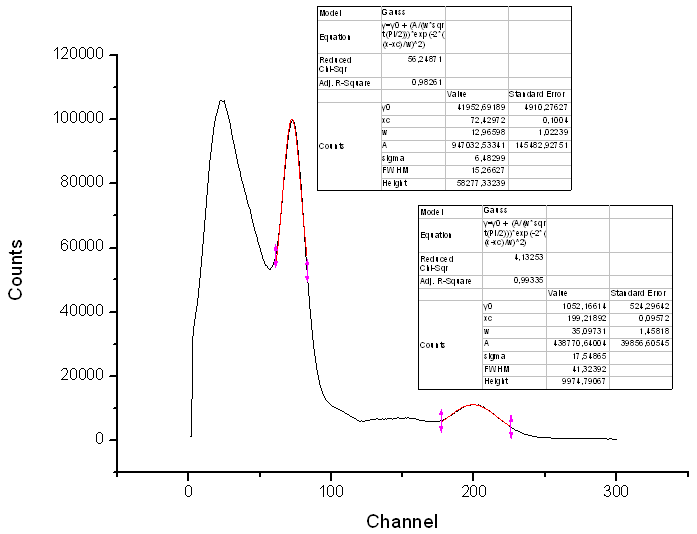
\includegraphics[height=0.3\textheight]{Graphen/SZ1.png}
 \caption{\Na-Spektrum mit SZ1}
\end{figure}

\begin{figure}
 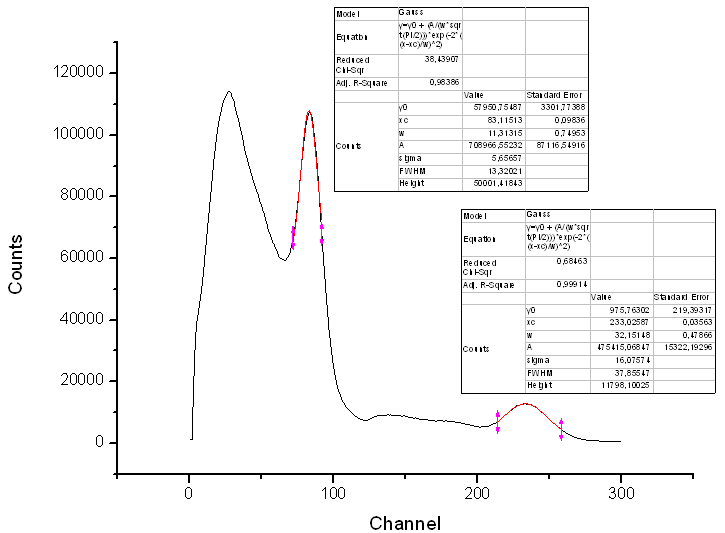
\includegraphics[height=0.3\textheight]{Graphen/SZ2.png}
 \caption{\Na-Spektrum mit SZ2}
\end{figure}

\begin{figure}
 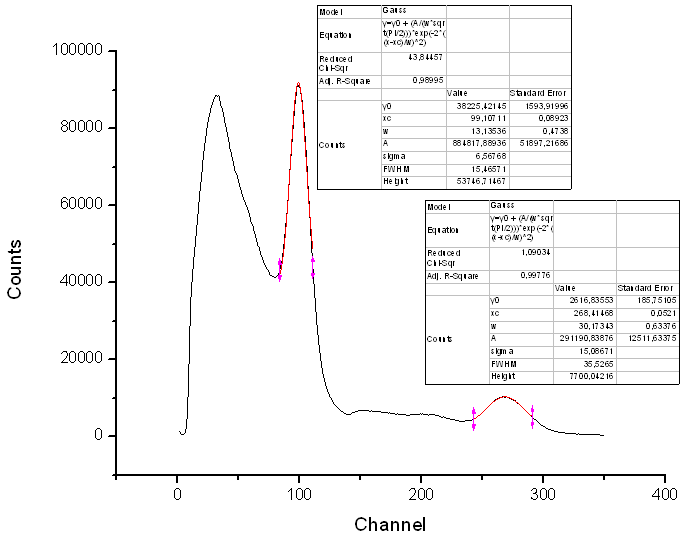
\includegraphics[height=0.3\textheight]{Graphen/SZ3.png}
 \caption{\Na-Spektrum mit SZ3}
\end{figure}  

Dazu haben wir, wie in Abb \ref{schaltplan_sca_lin_mca} dargestellt, das unipolare Signal des Verstärkers (AMP) zur Einstellung des Energiefensters am SCA verwendet. Liegt ein Ereigniss innerhalb dieses Fensters, so wird ein Signal an das Linear Gate gegeben. Dieses lässt dann für einen kurzen Moment das eigentliche (bipolare) Signal durch. Um die Verzögerung durch den SCA (mindestens ca. $0,05\mu s$) kompensieren zu können, wurde zwischen AMP und Linear Gate noch ein Delay eingebaut. Durch die Verzögerungseinstellung des SCA kann jetzt die Laufzeit beider Signale synchronisiert werden. Dazu wurden der positive Normausgang des SCA und der Ausgang des Delays an die Koinzidenz angeschlossen. Über die feinere Verzögerungseinstellung des SCA wurde die Zählrate maximiert. Anschließend wurden beide Signale an das Linear Gate angeschlossen und dessen Ausgangssignal mit dem MCA analysiert. Das genaue Anpassen der Signallaufzeiten ist wichtig, da sonst einerseits zufällige Ereignisse außerhalb des gewünschten Energiefensters gemessen werden, andererseits aber auch das eigentliche Signal abgeschnitten werden kann. Dies würde dann ebenfalls zu einer falschen Energiemessung führen.

Für eine erneute Messung des \Na-Spektrums haben wir folgende Einstellungen verwendet:
\begin{center}
\begin{tabular}{llll}
\toprule
 & SZ1 & SZ2 & SZ3\\
\midrule
Verstärkung & 8,12 & 10,0 & 10,0\\
Coarse Gain & 20 & 20 & 20\\
Shaping Time & 0,5 $\mu s$ & 0,5 $\mu s$ & 0,5 $\mu s$\\
Lower Level & 0,04 & 0,04 & 0,0\\
Upper Level & 10,02 & 10,02 & 10,0\\
Delay & 2,14 $\mu s$ & 1,83 $\mu s$ & 2,05 $\mu s$\\
Messdauer & 20 min & 20 min & 20 min\\
Delay SCA & 2 $\mu s$ & 2 $\mu s$ & 2 $\mu s$\\
\bottomrule
\end{tabular}
\end{center}

Aus den Spektren haben wir die Position der 511keV- und 1275keV-Peaks ermittelt:  
\begin{center}
\begin{tabular}{lcc}
\toprule
 & 511keV - Peak (Channel) & 1275 keV-Peak (Channel) \\
\midrule
SZ1 & $72,4 \pm 0,1$ & $199,2 \pm 0,1$ \\
SZ2 & $83,1 \pm 0,1$ & $233,0 \pm 0,03$ \\
SZ3 & $99,1 \pm 0,1$ & $268,4 \pm 0,1$ \\
\bottomrule 
\end{tabular}
\end{center}

Somit konnten wir eine Energie-Channel-Eichung für die drei Szintillatoren vornehmen:
\begin{center}
\begin{tabular}{ll}
\toprule
     & Energie-Channel-Eichung\\
\midrule
 SZ1 & $E = (6,03 \pm 0,01) keV \cdot c + (74,8 \pm 0.8) keV$\\
 SZ2 & $E = (5,097 \pm 0,004) keV \cdot c + (87,5 \pm 0,6) keV$\\
 SZ3 & $E = (4,513 \pm 0,004) keV \cdot c + (63,8 \pm 0,6) keV$\\
\bottomrule 
\end{tabular}
\end{center}

\subsection{Zwei-Photonen-Zerfall}

Beim Zerfall des 0S0-Singulett-Zustands des Positroniums können die Photonen, wie in der Theorie näher erläutert, nur in einem $180^\circ$-Winkel abgestrahlt werden. Dies wollen wir über eine Winkelkorrelationsmessung verifizieren. Dazu stellen wir die Szintilatoren auf ein 511keV Fenster ein und drehen SZ1 oder SZ3 gegen den festen SZ2. 

\begin{center}
\begin{tabular}{llll}
\toprule
 & SZ1 & SZ2 & SZ3\\
\midrule
Lower Level & 1,585 & 1,87 & 1,79\\
Upper Level & 2,940 & 3,05 & 3,07\\
511keV Peak & 81  & 80 & 94\\
\bottomrule
\end{tabular}
\end{center}

Die Position des 511keV Peaks zeigt also eine Abhängigkeit von der Einstellung der Energiefenster, insbesondere SZ1 mit $\Delta c_{511} = 8,6$. Dies könnte an einer falschen Delay-Einstellung liegen, der wir aber viel Zeit gewidmet haben, an der besseren Filterung durch den SCA oder an Defekten der Elektronik. Wir haben die Fenstereinstellung mit dem MCA und Computer "`auf Sicht"' vorgenommen und denken, dass wir den 511keV-Peak damit hinreichend genau einstellen konnten, auch wenn er nicht mit der vorher vorgenommenen Energieeichung übereinstimmt.

\subsubsection{SZ2 - SZ3}

Wir haben in $180^\circ$-Stellung von SZ2 und SZ3 die Koinzidenzrate mit der Koinzidenzeinheit optimiert. Dazu haben wir die Rate am Hex-Scaler betrachtet und die Delays angepasst.

\begin{center}
\begin{tabular}{llll}
 & Delay\\
SZ2 & 1,83 $\mu s$\\
SZ3 & 2,83 $\mu s$
\end{tabular}
\end{center}

Um den statistische Fehler möglichst klein zu halten (unter 2\%) berechnen wir die nötige Messzeit pro Winkeleinstellung. Bei $150^\circ$ beträgt die Zählrate etwa $n = 3 Hz$, sodass sich die nötige Dauer wie folgt berechnen läßt:
\begin{equation}
 0,02 = \frac{s_N}{N} = \frac{1}{\sqrt{N}} = \frac{1}{\sqrt{n t}} \Leftrightarrow t = \frac{1}{n}\left( \frac{s_N}{N} \right)^{-2} = 833,3s
\end{equation}
Dies entspricht $t \approx 13,89 \text{min}$. Wir wählen daher eine Messzeit von $t = 16,67 \text{min}$ pro Winkeleinstellung, da sich damit die 100Hz-Clock als Stoppsignal für den Hex-Scaler verwenden lässt (100 000 Counts). 

\begin{figure}
 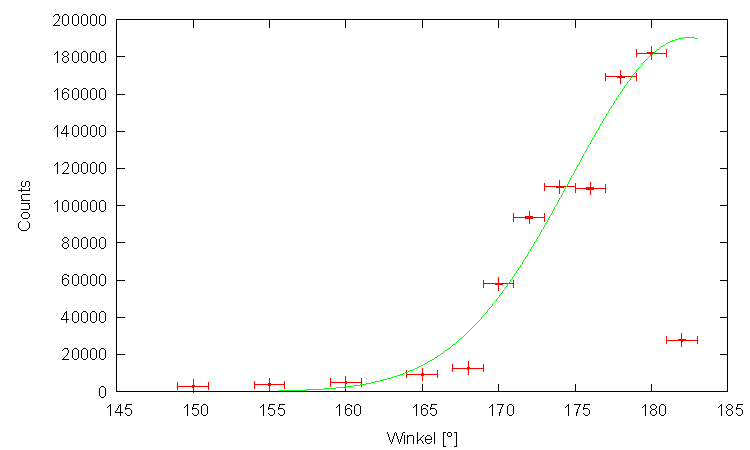
\includegraphics[width=\textwidth]{Graphen/2er/erste.pdf}
 \caption{Winkelkorrelation des Zwei-Photonen-Zerfalls (mit SZ2-SZ3}
\end{figure}

Bei einem Winkel von $182^\circ$ brach die Zählrate leider zusammen. Statt den erwarteten ca. 180 000 Counts erhielten wir nur noch 27 752, also einen Zusammenbruch um eine Größenordnung. Bei einer weiteren Messung stieg die Anzahl zwar wieder etwas, dennoch blieb sie in etwa halb so groß wie erwartet. Dies lag vor allem an einer Reduktion der Zählrate an SZ3 um einen Faktor 5.  

%TODO: Auswertung des Gauß-Fits
%TODO: Untergrund

\subsubsection{SZ2 - SZ1}

Um die Probleme mit SZ3 zu umgehen, haben wir eine erneute Messung mit SZ2-SZ1 durchgeführt. Dabei war die Koinzidenzrate deutlich höher als mit SZ2-SZ3 und somit nicht vergleichbar. Daher haben wir nochmals den kompletten Bereich von $150^\circ$ bis $210^\circ$ untersucht. Eine Messzeit von 100s erschien uns auf Grund der höheren Zählrate ausreichend. (Dies entspricht einem Fehler von ca. 5,8 \% bei $150^\circ$, bzw. 0,6\% bei $180^\circ$)

\begin{figure}
 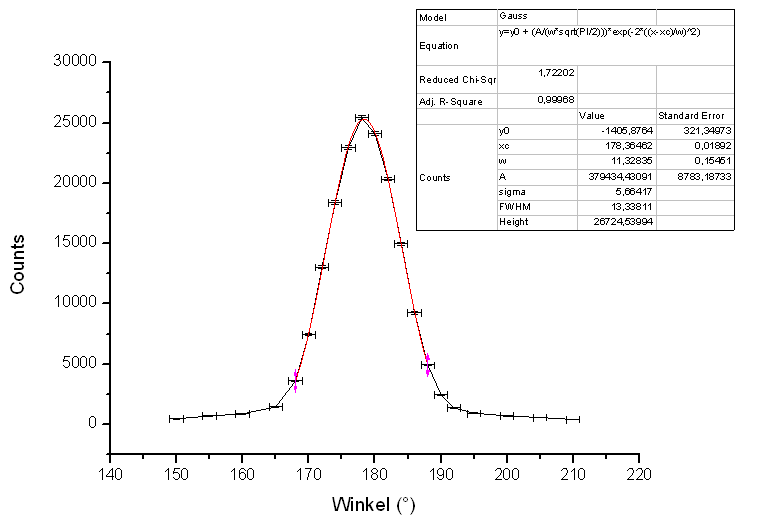
\includegraphics[width=\textwidth]{Graphen/180K.png}
 \caption{Winkelkorrelation des Zwei-Photonen-Zerfalls (mit SZ2-SZ1)}
\end{figure}

Unsere Messungen ergeben also, dass die maximale Zählrate bei $xc = 178,36^\circ \pm 0,01^\circ$ liegt und bestätigt somit die theoretische Aussage, dass der Zwei-Photonen-Zerfall nur in einem Winkel von $180^\circ$ erlaubt ist. Die "`Linienbreite"' von $w = 11^\circ \pm 0,15^\circ$ ergibt sich hauptsächlich aus der Bewegung des Schwerpunktsystems relativ zum Laborsystem. Das Positronium hat einen bestimmten Impuls der erhalten bleiben muss. Somit bewegt sich also das Schwerpunktsystem der beiden Photonen mit diesem weiter. Die resultierende 
%TODO: Abweichung von 180° erläutern

\subsubsection{Zufällige Koinzidenzen}

Um den Anteil der zufälligen Koinzidenzen, also Events die von zwei verschiedenen Zerfällen oder aus Störsignalen herrühren, zu bestimmen haben wir verschiedene Ansätze verfolgt. Zum Einen haben wir sie über die Zählraten und die Zeitauflösung der Koinzidenzeinheit abgeschätzt:
\begin{equation*}
 n_{ZK} = \tau \cdot n_{SZ2} \cdot n_{SZ3} = (0,1262 \pm 0,0057) s^{-1}
\end{equation*}

Weiterhin haben wir die Zahl der Koinzidenzen bei senkrechter Stellung der Szintillatoren gemessen:
\begin{equation*}
 n_{ZK-90} = (1,67  \pm  0,13) s^{-1}
\end{equation*}

Zu guter Letzt haben wir wieder die $180^\circ$-Konfiguration eingestellt und das Delay der beiden SCAs gegeneinander verstellt: 
\begin{equation*}
 n_{ZK-delay} = (0,019  \pm  0,004) s^{-1}
\end{equation*}

 
%TODO: was bedeutet das? größte verwenden?

\subsubsection{Austausch von SZ3}
Wir haben die gesamte Elektronik ausführlich untersucht und daraufhin den SCA von SZ3 ausgetauscht, da bei diesem der Pseudo-Peak bei ca 2000 keV viel stärker als bei den anderen beiden war. Weiterhin haben wir die Verstärkung am AMP etwas reduziert, da wir auch ein Übersteuern nicht ausschließen konnten. Danach war zwar das Signal deutlich klarer und der Pseudo-Peak verschwunden. Auf Grund der geänderten Verstärkereinstellungen wurde eine erneute Energie-Kanal-Eichung nötig, die in den Graphen des folgenden Kapitels mit abgebildet ist. 

\subsection{Drei-Photonen-Zerfall}

Bei diesem Versuchsteil geht es zuerst um die Untersuchung des Energiespektrums. Dazu haben wir die Fenster von SCA 1 (Abb \ref{graphen-3er-red-spektrum-sz1}) und SCA 3 (Abb \ref{graphen-3er-red-spektrum-sz3}) so eingestellt, dass nur Events unterhalb der 511keV-Linie registriert werden. Weiterhin haben wir die Signale aller Szintillatoren synchronisiert. Anschließend haben wir über den MCA das Energiespektrum von SZ2 aufgenommen. 
\begin{figure}
 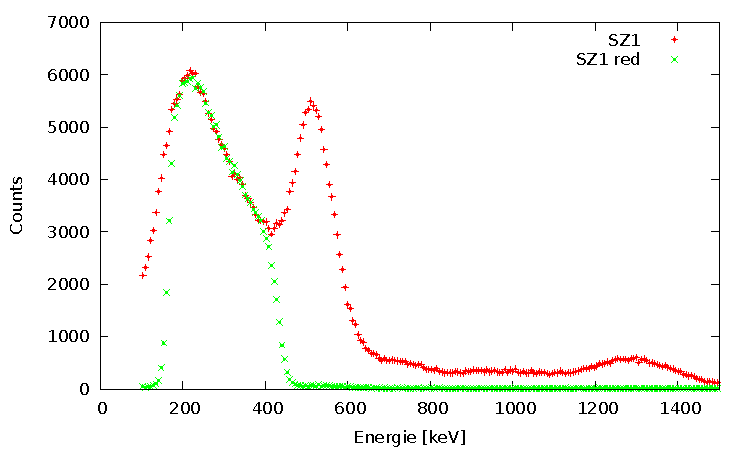
\includegraphics[width=\textwidth]{Graphen/3er/red-spektrum-sz1.pdf}
 \caption{Einstellung des Energiefensters unterhalb der 511keV-Linie für SZ1}
 \label{graphen-3er-red-spektrum-sz1}
\end{figure}


\begin{figure}
 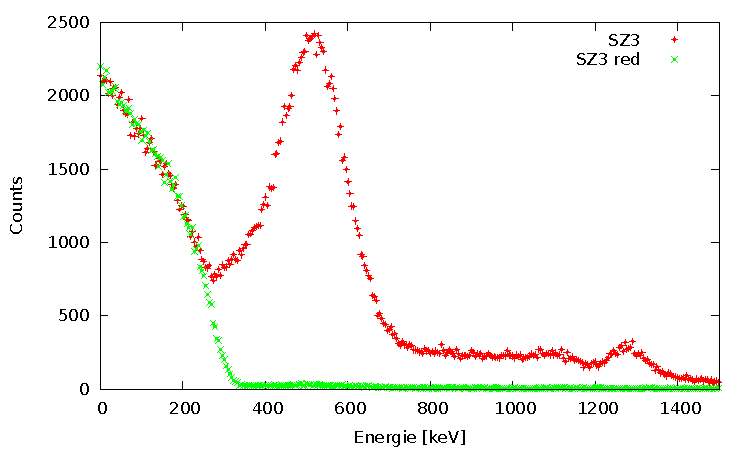
\includegraphics[width=\textwidth]{Graphen/3er/red-spektrum-sz3.pdf}
 \caption{Einstellung des Energiefensters unterhalb der 511keV-Linie für SZ3}
 \label{graphen-3er-red-spektrum-sz3}
\end{figure}

\begin{figure}
 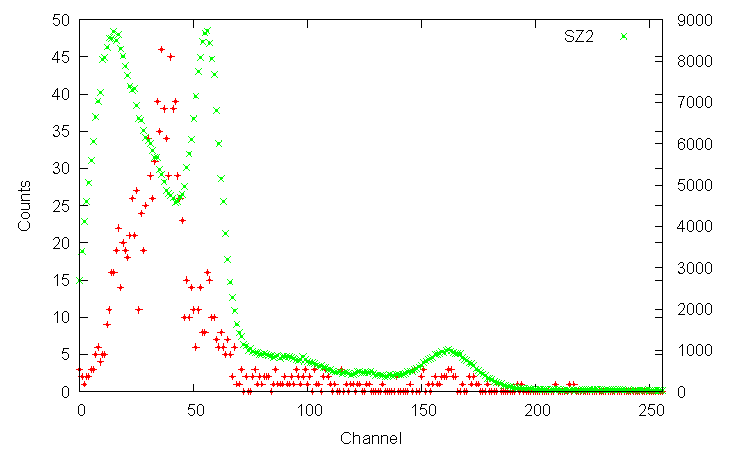
\includegraphics[width=\textwidth]{Graphen/3er/spektrum-2.pdf}
 \caption{Spektrum am SZ2 bei 3er-Koinzidenz}
 \label{graphen-3er-spektrum-2}
\end{figure}

Wir haben dazu eine Messung von ca. 3h Dauer (11091s) durchgeführt. Im Graphen (Abb \ref{graphen-3er-spektrum-2}) haben wir zum Vergleich auch das komplette \Na-Spektrum eingezeichnet. Das Spektrum zeigt ein relativ breites Maximum bei ca. $320-350 keV$. Dies entspricht also gut dem erwarteten Maximum bei $340 keV$, dass sich ergibt, wenn man die bei der Anihilation frei werdenende Energie auf drei Photonen zu gleichen Teilen aufteilt. Die Breite des Maximums entsteht dadurch, dass nicht nur genau die $120^\circ$-Konfiguration, sondern auch ähnliche ein zulässiges Event produzieren.

%TODO: Parameter?

\begin{figure}
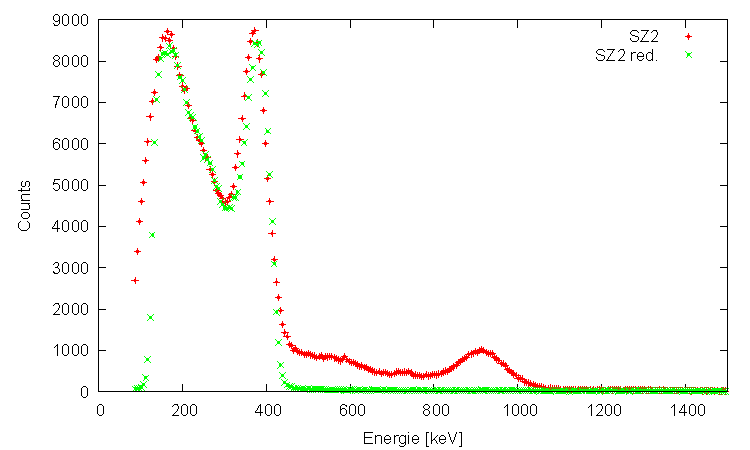
\includegraphics[width=\textwidth]{Graphen/3er/red-spektrum-sz2.pdf}
 \caption{Grobe Einstellung des Energiefensters von SZ2}
\label{graphen-3er-red-spektrum-sz2}
\end{figure}

Für die weiteren Messungen haben wir auch bei SZ2 ein Energiefenster eingestellt, allerdings nur recht grob da die Zählrate auch so schon niedrig war (Abb \ref{graphen-3er-red-spektrum-sz2}). Statt eventuell zulässige Ereignisse von vorneherein zu unterdrücken, haben wir dann lieber bei der Auswertung die Daten etwas beschnitten.

Aus den erneut aufgenommenen \Na-Spektren haben wir die Position der 511keV- und 1275keV-Peaks abgelesen:  
\begin{center}
\begin{tabular}{lcc}
\toprule
 & 511keV - Peak (Channel) & 1275 keV-Peak (Channel) \\
\midrule
SZ1 & $64,04 \pm 0,07$ & $184,2 \pm 3,4$ \\
SZ2 & $55,25 \pm 0,06$ & $161,54 \pm 0,17$ \\
SZ3 & $183,2 \pm 0,2$ & $351,6 \pm 0,6$ \\
\bottomrule 
\end{tabular}
\end{center}

Somit konnten wir eine Energie-Channel-Eichung für die drei Szintillatoren vornehmen:

\begin{center}
\begin{tabular}{ll}
\toprule
     & Energie-Channel-Eichung\\
\midrule
 SZ1 & $E = (6,36 \pm 0,18) keV \cdot c + (103,7 \pm 11,6) keV$\\
 SZ2 & $E = (7,19 \pm 0,01) keV \cdot c + (113,9 \pm 0,8) keV$\\
 SZ3 & $E = (4,54 \pm 0,02) keV \cdot c + (-320,4 \pm 3,2) keV$\\
\bottomrule 
\end{tabular}
\end{center}

Dabei fällt bei SZ3 (Abb \ref{graphen-3er-red-spektrum-sz3}) auf, dass angeblich einige Kanäle des MCA Photonen mit negativer Energie gemessen haben. Dies ist eher unwahrscheinlich und wir vermuten daher zwei Hauptfehlerquellen: einerseits könnten wir die Peaks verwechselt haben. Der 511 keV-Peak müsste dann in der abfallenden Flanke der Bremsstrahlung "`versteckt sein"' (momentan ca. 200keV) und der 1275keV Peak wäre dann der von uns als 511keV angenommene. Die gute Übereinstimmung des Kurvenverlaufs spricht allerdings eher gegen diese These. Eine andere Möglichkeit wäre eine Nichtlinearität, vermutlich bereits direkt in SZ3 oder eventuell auch im Verstärker. Diese erscheint uns wahrscheinlicher. Sollten wir allerdings tatsächlich die Peaks verwechselt haben, würde dies zwar die weitere Messgenauigkeit verschlechtern und zusätzliche Ereignisse erzeugen, nicht jedoch gültige Ereignisse verwerfen. Für die weitere Auswertung haben wir die Annahme getroffen, dass sich die Energie-Kanal-Einstellung auch im Bereich 0-551 keV linear ändert und haben Kanal 0 mit 0keV identifiziert. Es ergibt sich dann folgende (grobe) Energie-Kanal-Eichung:

\begin{equation}
 E(c) = \begin{cases}
 ( 2,79 \pm 1,7) keV \cdot c + (0 \pm 70) keV & c < 183 \\
 (4,54 \pm 0,02) keV \cdot c + (-320,4 \pm 3,2) keV & c \geq 183
 \end{cases}
\end{equation}


\subsection{Quenching}

Beim Quenching untersuchen wir die Abnahme des Drei-Photonen-Zerfalls unter zunehmendem Magnetfeld. Dazu haben wir zweistündige Messungen mit konstantem Magnetfeld durchgeführt und nach je zwei Messungen eine Kontrollmessung ohne Magnetfeld. Diese erlaubt es uns, grobe Drifts und Schwankungen in der Messung zu erkennen und zu kompensieren. Im Anschluss haben wir das Delay von SZ1 verändert. Mit einer weiteren Messung konnten wir sodie Zahl der zufälligen Koinzidenzen ermitteln.

% \begin{figure}
%  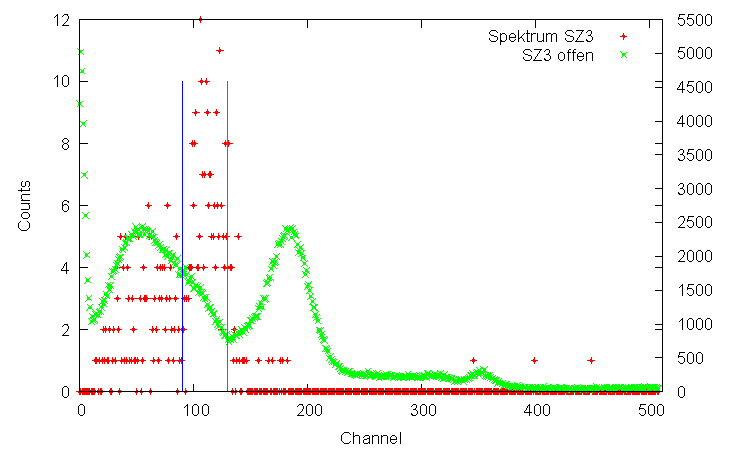
\includegraphics[width=\textwidth]{Graphen/quench/spektrum_0-3.pdf}
%  \caption{Spektrum 0,3A}
% \end{figure}

\begin{figure}
 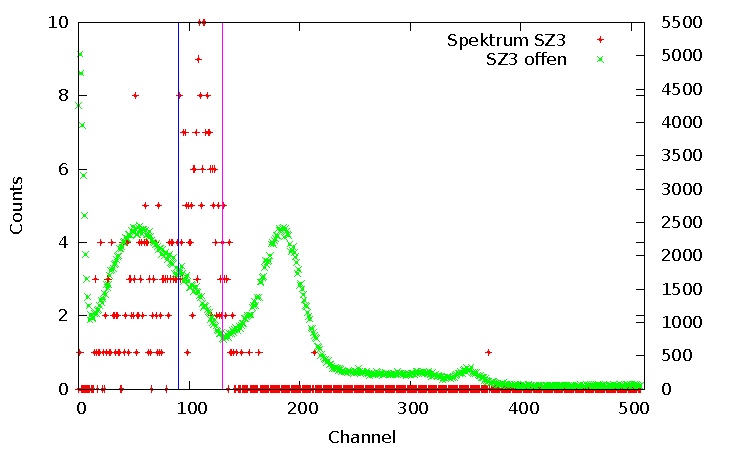
\includegraphics[width=\textwidth]{Graphen/quench/spektrum_1065.pdf}
 \caption{Spektrum 1065G}
\end{figure}


% \begin{figure}
%  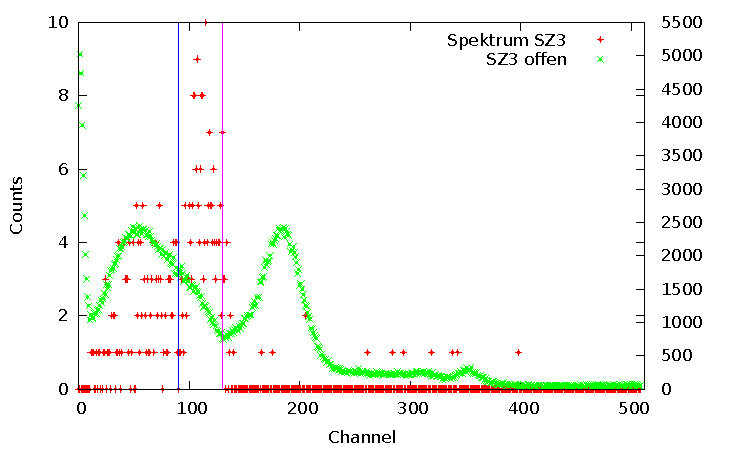
\includegraphics[width=\textwidth]{Graphen/quench/spektrum_2028.pdf}
%  \caption{Spektrum 2028G}
% \end{figure}
% 
% 
% \begin{figure}
%  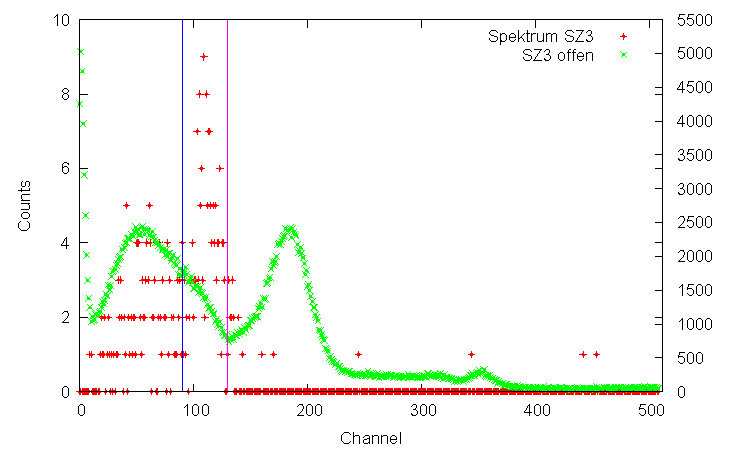
\includegraphics[width=\textwidth]{Graphen/quench/spektrum_3070.pdf}
%  \caption{Spektrum 3070G}
% \end{figure}
% 
% \begin{figure}
%  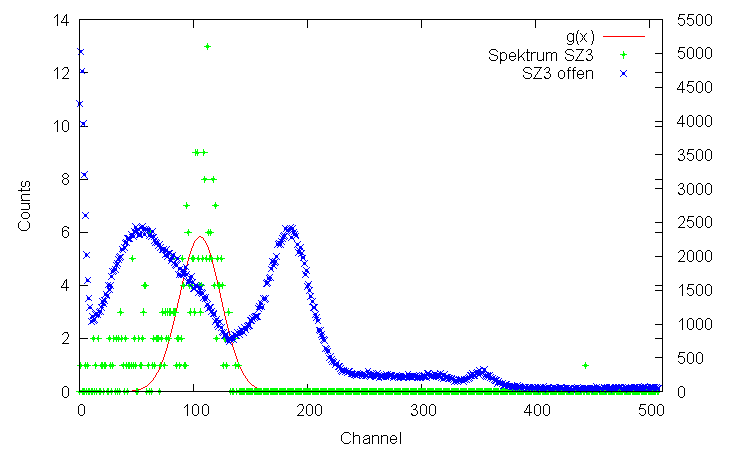
\includegraphics[width=\textwidth]{Graphen/quench/spektrum_4032.pdf}
%  \caption{Spektrum 4032G}
% \end{figure}

%\begin{figure}
% 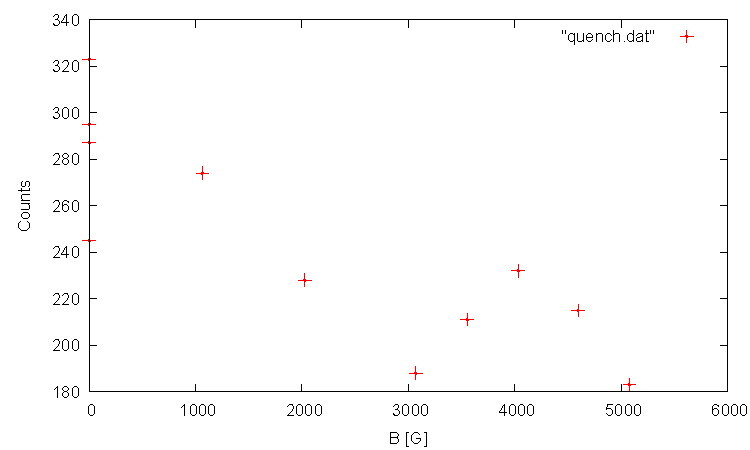
\includegraphics[width=\textwidth]{Auswertung/quench.pdf}
% \caption{Quenching des Drei-Photonen-Zerfalls in $120^\circ$-Konfiguration}
%\end{figure}

Bei der Auswertung haben wir dann nur die Kanäle 90 bis 130 verwendet, was einem Energiefenster von 250 bis 365 keV entspricht. Die Ereignisse in diesem Intervall haben wir dann summiert und den Untergrund (2 zufällige Koinzidnezen in 2h) aus der Koinzidenzmessung abgezogen. Um die Schwankungen in der Apparatur auszugleichen, die uns die Kontrollmessungen zeigen, haben wir zur Normierung ein gewichtetes Mittel dieser verwendet.
\begin{equation*}
 N' = \frac{N}{2/3 N_{k1} + 1/3 N_{k2}}
\end{equation*}
Wobei $N_{k1}$ die zeitlich näherliegende Kontrollmessung bezeichnet und $N_{k2}$ die weiter entfernte. An die resultierenden Datenpunkte haben wir dann die Quenching-Funktion über den Parameter $\Delta W$ angepasst:
\begin{equation*}
 Q(B)/Q(0) = 0.5 + \frac{0.5}{1 + r \cdot ( \frac{2  \mu }{ \Delta W})^2 \cdot B^2} 
\end{equation*}

Im Graph (Abb \ref{auswertung-quench-normiert}) ist sowohl ein Fit an die Datenpunkte dargestellt, die über das gewichtete Mittel normiert wurden (f(x)) als auch ein Fit an Datenpunkte, die mit dem durchschnittlichen $Q(0)$ normiert wurden. 



\begin{figure}
 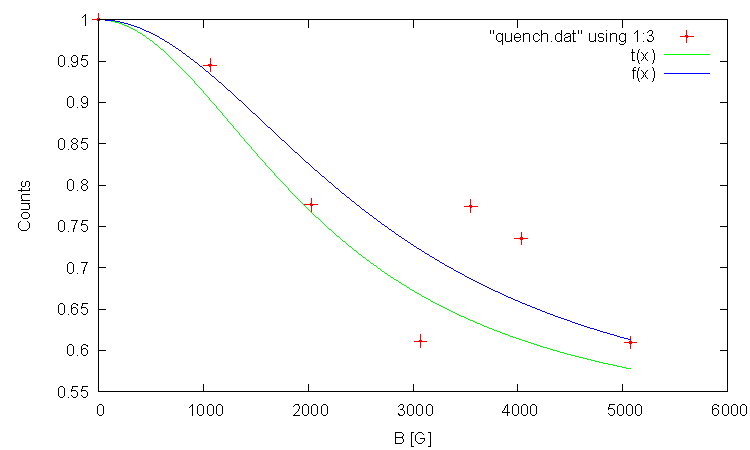
\includegraphics[width=\textwidth]{Auswertung/quench-normiert.pdf}
 \caption{Normiertes Quenching des Drei-Photonen-Zerfalls in $120^\circ$-Konfiguration}
 \label{auswertung-quench-normiert}
\end{figure}

Wir erhalten aus dem Fit folgenden Wert für die Feinstrukturaufspaltung:
\begin{equation*}
 \Delta W = (9,068 \pm 0,66) \e{-4} eV
\end{equation*}

Der Literaturwert beträgt $\Delta W = 8,412\e{-4} eV$ und liegt also innerhalb der ersten Standardabweichung des von uns ermittelten Wertes. Die relativen Zählraten sind bei mehreren Einstellungen zu hoch. Dies deutet darauf hin, dass falsche Ereignisse registriert werden, also zB von 2-Photonen-Zerfällen, Bremsstrahlung oder auch Rauschen. Diese werden nicht vom Magnetfeld unterdrückt und führen somit zu einer zu großen Zählrate. Theoretisch ließen sich solche Ereignisse weiter reduzieren, indem engere Energiefenster und auch ein kleineres Koinzidenzintervall gewählt werden. Praktisch müsste dann allerdings die Meßzeit noch weiter verlängert werden, um statistisch relevante Ergebnisse zu erhalten. Da wir aber bereits so deutliche Drifts in den Messwerten sehen, scheint dies nicht sinnvoll. Besser wäre es sicherlich die \Na-Probe zu erneuern, wodurch sich ca. 100-fach höhere Zählraten ergeben würden (siehe \ref{verbleibende_aktivitaet}).

Eine weitere Fehlerquelle ist natürlich das Magnetfeld, bzw. die Spule die es erzeugt. So zeigte sich während den Messungen ein Absinken der Stromstärke um bis zu 2\%. Weiterhin ist die Eichtabelle schon fast 30 Jahre alt, was uns dazu veranlasst hat diese mit einer Hall-Sonde zu kontrollieren. Die Ergebnisse liegen systematisch ca. 1,6 \% über den tabellierten Werten. Da sich beide Fehler also im Endeffekt kompensieren, haben wir die tabellierten Werte verwendet und einen Fehler von 2\% angenommen. Die Messwerte sind in der folgenden Tabelle nochmals zusammengefasst: 

\begin{tabular}{lllll}
\toprule
I [A] & $B_{2011}$ [G] & $B_{1981}$ [G] & $\Delta B$ [G] \\
\midrule
0,03&	56,2&	0&	56,2\\
5&	2050&	2028&	22\\
7,6&	3120&	3070&	50\\
10&	4100&	4032&	68\\
12,6&	5120&	5075&	45\\
8,8&	3620&	3551&	69\\
11,4&	4650&	4594&	56\\
9,78&	4020&	3952&	68\\
10,68&	4360&	4280&	80\\
9,13&	3750&	3680&	70\\
10,47&	4280&	4200&	80\\
\bottomrule
\end{tabular}

\section{Zusammenfassung}

\section{Appendix}

\begin{appendix}
\section{Sources}

\begin{itemize}
\item Baur, C. : \emph{Einrichtung des Versuches ''Optisches Pumpen mit Laserdioden''}, Freiburg im Breisgau 1997 [Ba97]
\item Moseler, M., Pfaff, O. : \emph{Optisches Pumpen}, Freiburg im Breisgau 1990
\item Demtröder, W.: \emph{Experimentalphysik 3: Atome, Moleküle und Festkörper}, Kaiserslautern 2005
\end{itemize}

\end{appendix}

\clearpage

\section{Protocol}

\clearpage

%\bibliographystyle{alphadin} 
%\bibliography{bib}


\end{document}
